\documentclass{beamer}
\usetheme{madrid}

\usepackage{ctex}
\usepackage{color}
\usepackage{tikz}
\usetikzlibrary{positioning, shapes.geometric}
\usepackage{graphicx}

\usepackage{advdate}

\hypersetup{pdfpagemode=FullScreen}

\title{空间辐射场三维重构方法}
\author[刘铭]{%
    刘铭\\
    导师:宋玉收%
}
\institute{哈尔滨工程大学核科学与技术学院}
\date{\AdvanceDate[+1]\today}

\begin{document}

\begin{frame}
    \maketitle
\end{frame}

\begin{frame}
    \tableofcontents
\end{frame}

\section{选题回顾}

\begin{frame}{选题回顾}
    空间辐射场三维重构方法是\textcolor{blue}{辐射场可视化仿真技术}的一项重要技术。辐射场可视化仿真技术不仅能够应用在\textcolor{red}{核设施退役工程},将辐射场的分布以可视化的形式显示在虚拟场景中,评估施工人员所接受的辐射剂量;还能在\textcolor{red}{核与辐射安全科普}工作中发挥积极的作用,将辐射场的剂量值、分布等定量信息展现给公众,易于科普工作者与公众进行互动沟通,提高公众对核科学的认识。
\end{frame}

\section{已完成工作}

\subsection{调研所得内容}
\begin{frame}{调研所得内容}
    辐射场重构方法:
    \begin{enumerate}
        \item "正演"方法
              \note{“正演”方法是通过对辐射传输方程进行求解,在了解放射源基本信息的基础上,构造准确的系统模型进行粒子运输模拟,从而将空间辐射场进行重构}
              \begin{itemize}
                  \item 蒙特卡洛法
                        \begin{enumerate}
                            \item MCNP
                                  \note{美国洛斯阿拉莫斯国家实验室开发的蒙特卡洛辐射输运软件 }
                            \item Geant4
                                  \note{欧洲核子研究组织开发的蒙特卡洛应用软件包}
                            \item SuperMC
                                  \note{中科院核能安全技术研究所开发的核设计与辐射安全评价软件}
                        \end{enumerate}
                  \item 点核积分法
                        \begin{enumerate}
                            \item Narveos
                                  \note{法国国家能源局开发的用于核辐射工作场所的虚拟现实仿真软件}
                            \item VISIPLAN
                                  \note{比利时核研究中心开发的剂量评估软件}
                        \end{enumerate}
              \end{itemize}
        \item "反演"方法
              \note{“反演”方法是在未知放射源基本信息的情况下,通过实际测量获得有限、离散的采样数据进行分析和空间重构,从而获得完整的辐射场分布数据}
              \begin{itemize}
                  \item 插值方法
                        \begin{enumerate}
                            \item 径向基插值RBF(样条插值)
                            \item 反距离权重法IDW(克里金插值)
                        \end{enumerate}
                  \item 拟合方法
                        \begin{enumerate}
                            \item 最小二乘法
                            \item 最小立方法
                        \end{enumerate}
              \end{itemize}
    \end{enumerate}
\end{frame}

\subsection{插值算法学习}
\begin{frame}{样条插值}
    样条函数是一种分段多项式,且相邻多项式之间具有一定的连续性。因此,样条函数既具有多项式的使用优点,又保留了各段之间的独立性。
    \begin{equation*}
        f(x,y,z)=\sum_{i=0}^{3}\sum_{j=0}^{3}\sum_{k=0}^{3}B_{i}(r)B_{j}(s)B_{k}(t) \phi_{(a+i)(b+j)(c+k)}
    \end{equation*}
    \begin{figure}
        \centering
        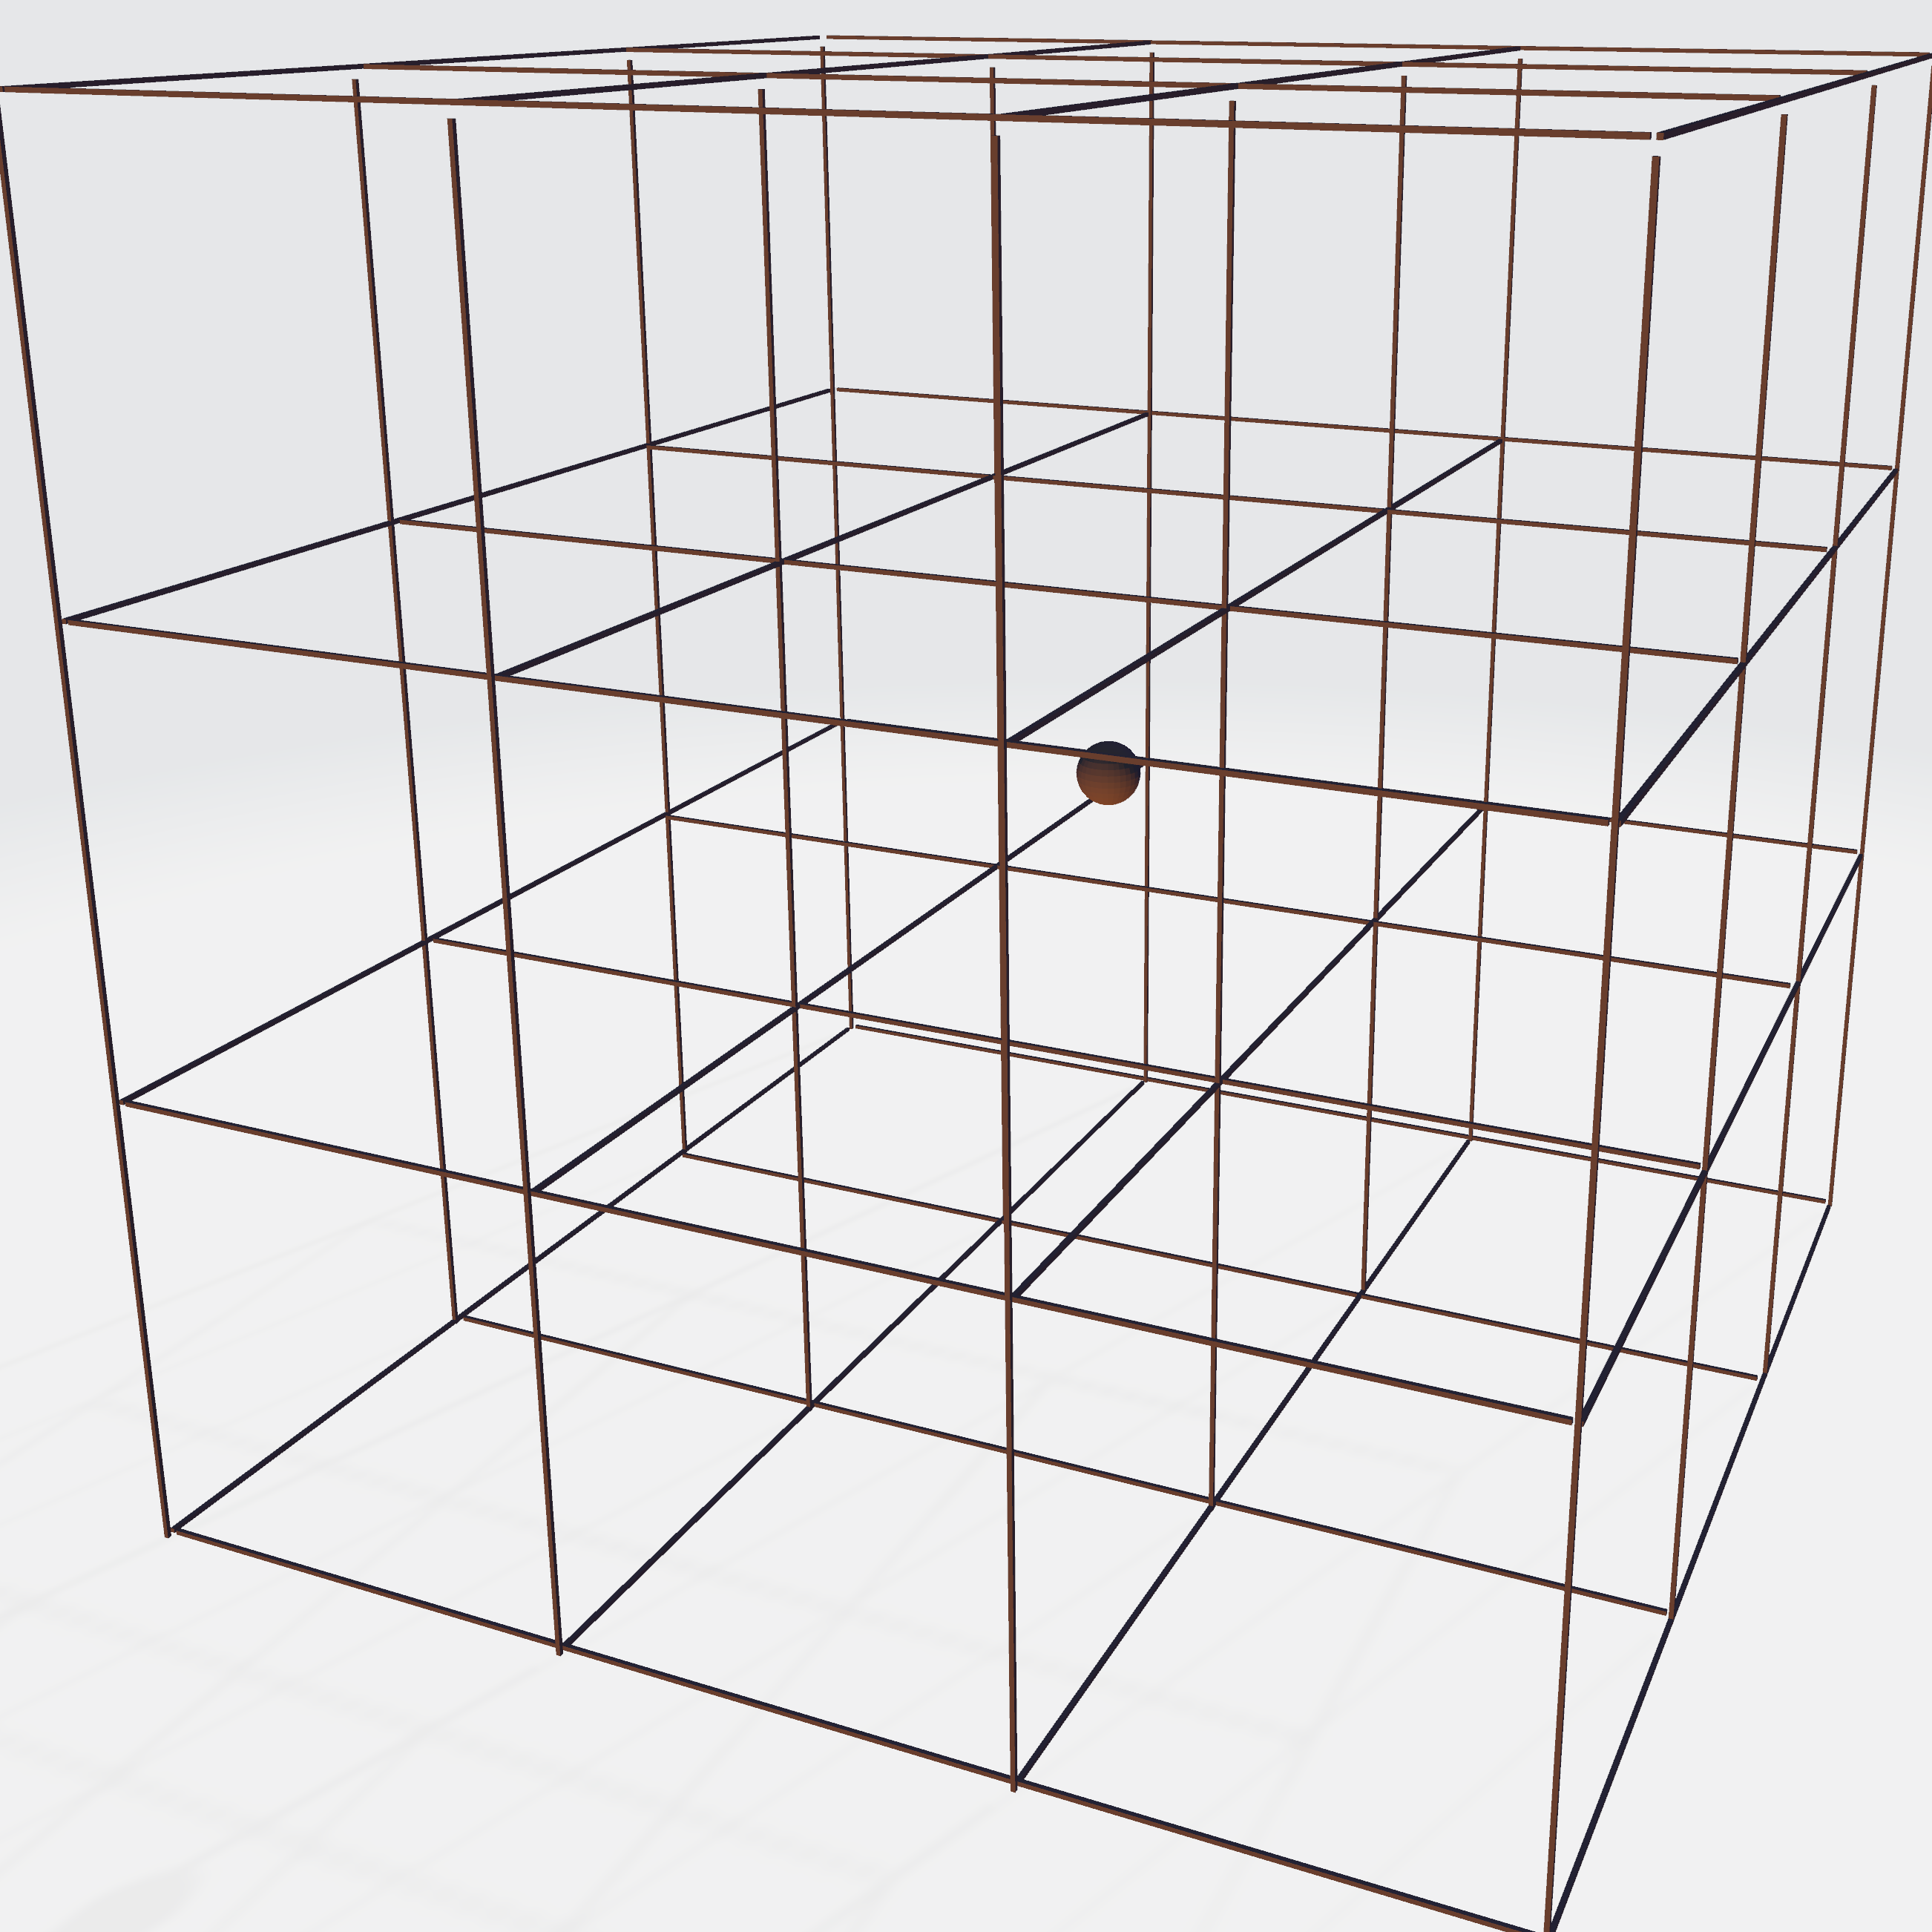
\includegraphics[width=0.4\textwidth]{3D B-splines.png}
    \end{figure}
\end{frame}

\begin{frame}{克里金插值}
    反距离权重法:彼此距离较近的事物要比彼此距离较远的事物更相似!
    \begin{equation*}
        \hat{v} = \sum_{i=1}^{n} \frac{1}{d^{p}}v_{i}
    \end{equation*}
    克里金插值:相比于距离反比加权算法具有更高的计算精度、计算效率以及计算复杂程度:
    \begin{equation*}
        \hat{v_{o}} = \sum_{i=1}^{n}\lambda_{i}v_{i}
    \end{equation*}
    克里金模型:普通克里金、简单克里金、泛克里金、概率克里金、析取克里金、指示克里金、协同克里金等
\end{frame}

\subsection{提出创新思路}
\begin{frame}{提出创新思路}
    空间插值的确定性方法包含\textcolor{blue}{反距离权重法 IDW(克里金插值)} 以及\textcolor{blue}{径向基函数插值法 RBF(B 样条插值)} 等,但仅仅\textcolor{red}{依靠某种单一的方法难以对辐射场重构的很好}。因此提出一种新的重构方法,将两种插值的结果进行对比,对于重构出来的两个不同的辐射场,将重构出来的两个辐射场剂量值相差较大的区域,选点进行再次测量,从而最终得到重构辐射场,相比于依靠某单一插值方法,随机选取同样的测量点进行重构插值得到的辐射场,应该会有更好的效果。
\end{frame}

\subsection{重构方法程序}
\begin{frame}{重构方法程序}
    \begin{tikzpicture}[node distance=5pt]
        \node[draw, rounded corners]                        (start)   {开始};
        \node[draw, below=of start]                         (step 1)  {导入数据};
        \node[draw, below=of step 1]                        (step 2)  {计算Kriging插值重构辐射场};
        \node[draw, below=of step 2]                        (step 3)  {计算Splines插值重构辐射场};
        \node[draw, below=of step 3]                        (step 4)  {计算两个重构辐射场的偏差};
        \node[draw, diamond, aspect=6, below=of step 4]     (choice)  {偏差值是否大于设定值};
        \node[draw, right=20pt of choice]                   (step x)  {添加测量数据};
        \node[draw, below=8pt of choice]                   (step 5)  {绘制空间辐射场};
        \node[draw, below=of step 5]                        (step 6)  {计算整体偏差};
        \node[draw, rounded corners, below=of step 6]       (end)     {结束};

        \draw[->] (start)  -- (step 1);
        \draw[->] (step 1) -- (step 2);
        \draw[->] (step 2) -- (step 3);
        \draw[->] (step 3) -- (step 4);
        \draw[->] (step 4) -- (choice);
        \draw[->] (choice) -- (step 5);
        \draw[->] (choice) -- node[left]  {否} (step 5);
        \draw[->] (choice) -- node[above] {是}  (step x);
        \draw[->] (step 5) -- (step 6);
        \draw[->] (step x) -- (step x|-step 1) -> (step 1);
        \draw[->] (step 6) -- (end);
    \end{tikzpicture}
\end{frame}

\section{后续工作}
\begin{frame}{后续工作}
    \begin{enumerate}
        \item 获取辐射场数据
              \begin{itemize}
                  \item 实验测量
                  \item Geant4仿真
                  \item 点核积分法
              \end{itemize}
        \item 比较创新重构方法与单一方法重构的辐射场与实际辐射场的插值重构效果
              \begin{itemize}
                  \item 单源情况
                  \item 多源情况
                  \item 简单空间
                  \item 复杂空间
              \end{itemize}
    \end{enumerate}
\end{frame}

\begin{frame}
    \Huge{\centerline{谢谢!}}
\end{frame}

\end{document}